\documentclass[tikz,12pt]{standalone}
\usepackage{textcomp}

\usepackage{tikz}
\usetikzlibrary{shapes.geometric, arrows}
\usepackage{xcolor}

% Custom colors
\definecolor{backcolour}{rgb}{0.95,0.95,0.92}
\definecolor{backcolour}{RGB}{229, 229, 229}
% Polar Night Palette
\definecolor{nightDarkest}{RGB}{46, 52, 64}
\definecolor{nightDark}{RGB}{59, 66, 82}
\definecolor{nightMid}{RGB}{67, 76, 94}
\definecolor{nightLight}{RGB}{76, 86, 106}
% Snow Storm Palette
\definecolor{snowDark}{RGB}{216, 222, 233}
\definecolor{snowMid}{RGB}{229, 233, 240}
\definecolor{snowLight}{RGB}{236, 239, 244}
% Frost Palette
\definecolor{frostTurqoise}{RGB}{143, 188, 187}
\definecolor{frostLightBlue}{RGB}{136, 192, 208}
\definecolor{frostMidBlue}{RGB}{129, 161, 193}
\definecolor{frostDarkBlue}{RGB}{94, 129, 172}
% Aurora Palette
\definecolor{auroraLila}{RGB}{180, 142, 173}
\definecolor{auroraRed}{RGB}{191, 97, 106}
\definecolor{auroraOrange}{RGB}{208, 135, 112}
\definecolor{auroraYellow}{RGB}{235, 203, 139}
\definecolor{auroraGreen}{RGB}{163, 190, 140}

% Baskervald X for roman, with oldstyle figure
\usepackage[osf]{Baskervaldx}
% load amssymb before newtxmath to avoid problem with \Bbbk
\usepackage{amssymb}
% Nice math calligraphic font 
\usepackage[cal=boondoxo]{mathalpha}
% Math font to match
\usepackage[bigdelims,baskervaldx]{newtxmath}

\begin{document}


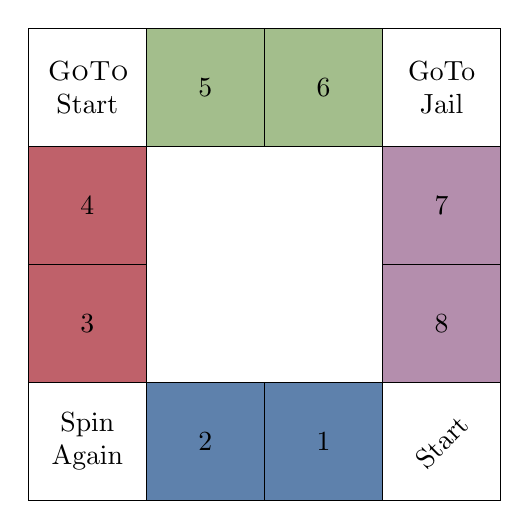
\begin{tikzpicture}
    [
        node distance=1.5cm,
        place/.style={
            draw, rectangle, minimum size=1.5cm, text width=1cm,
            align=center
        }
    ]

% Nodes
\node (start) [place] {\rotatebox{45}{Start}};

\node (one) [
		place, left of=start, fill=frostDarkBlue,
    ] {1}; 

\node (two) [
		place, left of=one, fill=frostDarkBlue,
	] {2};

\node (roll-again) [
		place, left of=two, text width=1cm,
	] {Spin Again};

\node (three) [
		place, above of=roll-again, fill=auroraRed,
	] {3};

\node (four) [
		place, above of=three, fill=auroraRed,
	] {4};

\node (goto-start) [
        place, above of=four
	] {\textsc{GoTo} Start};

\node (five) [
		place, right of=goto-start, fill=auroraGreen,
    ] {5};

\node (six) [
		place, right of=five, fill=auroraGreen,
	] {6};
    
\node (goto_jail) [
        place, right of=six
    ] {GoTo Jail};

\node (seven) [
		place, below of=goto_jail, fill=auroraLila,
    ] {7};

\node (eight) [
		place, below of=seven, fill=auroraLila,
	] {8};

\end{tikzpicture}
\end{document}
